% Copyright 2021 Fausto Spoto
%
% Licensed under the Apache License, Version 2.0 (the "License");
% you may not use this file except in compliance with the License.
% You may obtain a copy of the License at
%
%    http://www.apache.org/licenses/LICENSE-2.0
%
% Unless required by applicable law or agreed to in writing, software
% distributed under the License is distributed on an "AS IS" BASIS,
% WITHOUT WARRANTIES OR CONDITIONS OF ANY KIND, either express or implied.
% See the License for the specific language governing permissions and
% limitations under the License.

\documentclass[11pt]{beamer}  %% versione proiettore
%%\documentclass[11pt,handout]{beamer} %% versione stampa
\usepackage{lucidiJb-2ed}
\usepackage{mathtools}
\usepackage{relsize}

\mode<article>
{
  \usepackage{fullpage}
  \usepackage{hyperref}
}

\mode<presentation>
{
  \setbeamertemplate{background canvas}[vertical shading][bottom=red!10,top=blue!10]
  \usetheme{Course}
  \usefonttheme[onlysmall]{structurebold}
}

\subtitle{Blockchain Course}
\title{Tendermint}
\institute{Universit\`a di Verona, Italy}
\date{February 2021}

\setbeamercovered{invisible}

\def\codesize{\smaller}
\def\<#1>{\codeid{#1}}
\newcommand{\codeid}[1]{\ifmmode{\mbox{\codesize\ttfamily{#1}}}\else{\codesize\ttfamily #1}\fi}

\begin{document}

\begin{frame}
  \titlepage
\end{frame}

\begin{frame}
  \frametitle{Proof of\ldots}

  \begin{center}
    Who decides the next block?
  \end{center}

  \bigskip

  \begin{greenbox}{Proof-of-work [PoW] is expensive and leads to forks}
    \begin{itemize}
    \item proof-of-stake [PoS] (who owns the most)
    \item proof-of-space (who consumed more memory)
    \item proof-of-authority (who has more authority)
    \item \ldots
    \end{itemize}
  \end{greenbox}

  \bigskip

  \begin{greenbox}{PoS is a variant of Practical Byzantine Fault Tolerance (BFT)}
    Miguel Castro and Barbara Liskov.
    \emph{Practical Byzantine Fault Tolerance and Proactive Recovery}.
    ACM Trans.\ Comput.\ Syst., 20(4):398–461, November 2002
  \end{greenbox}

\end{frame}

\begin{frame}\frametitle{Tendermint}

  \begin{greenbox}{Jae Kwon. \emph{Tendermint: Consensus without Mining}, 2014.\\
    \url{https://tendermint.com/static/docs/tendermint.pdf}}
    \begin{itemize}
    \item a dynamic set $V$ of validators decides the next block
    \item $V$ might be different for each block
      \begin{itemize}
      \item but deterministically computed from the previous history
      \end{itemize}
    \item at each height $H$, each validator $v\in V$:
      \begin{enumerate}
      \item identifies (deterministically) a validator $p\in V$ that
        is expected to aggregate some transactions and \alert{propose} a next block $b$
      \item if it considers $b$ valid, it \alert{pre-votes} $b$
      \item counts how many validators pre-vote $b$
      \item if it counted at least $\frac{2}{3}$ pre-votes, it \alert{pre-commits} $b$
      \item counts how many validators pre-commit $b$
      \item if it counted at least $\frac{2}{3}$ pre-commits, it \alert{commits} $b$ and increases $H$
      \item goes back to step~1
      \end{enumerate}
    \end{itemize}
  \end{greenbox}

  \smallskip

  \begin{center}
    Tendermint is BFT. If step~1 is based on stakes, then it is PoS
  \end{center}

\end{frame}

\begin{frame}\frametitle{The mempool}

  \begin{center}
    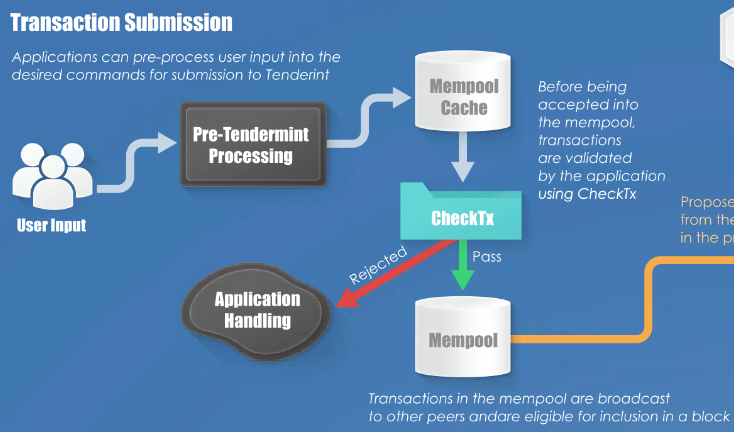
\includegraphics[scale=.4,clip=false]{pictures/tendermint-mempool.png}
  \end{center}

  \begin{center}
    \<checkTx(tx)> checks if the transaction \<tx> is valid
  \end{center}

\end{frame}

\begin{frame}\frametitle{Pre-vote}

  \begin{center}
    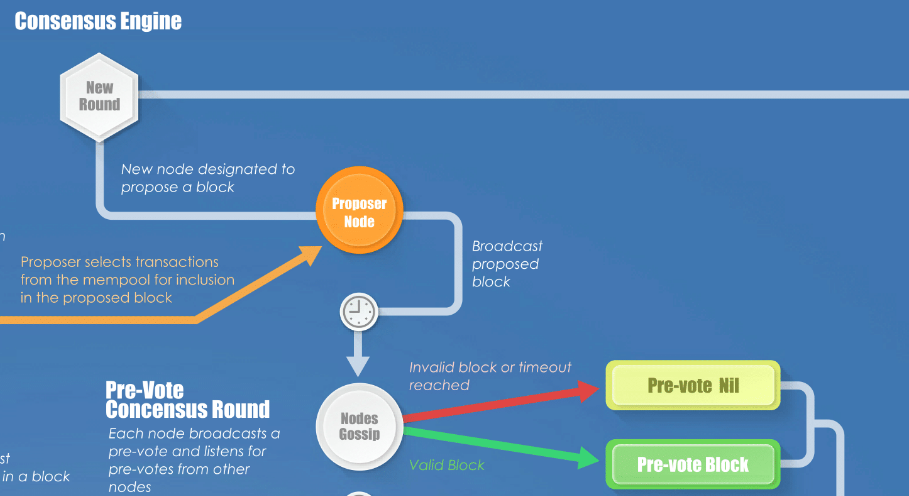
\includegraphics[scale=.38,clip=false]{pictures/tendermint-prevote.png}
  \end{center}

  \begin{center}
    \<checkTx(tx)> again to check if the transactions in the block are valid
  \end{center}

\end{frame}

\begin{frame}\frametitle{Pre-commit}

  \begin{center}
    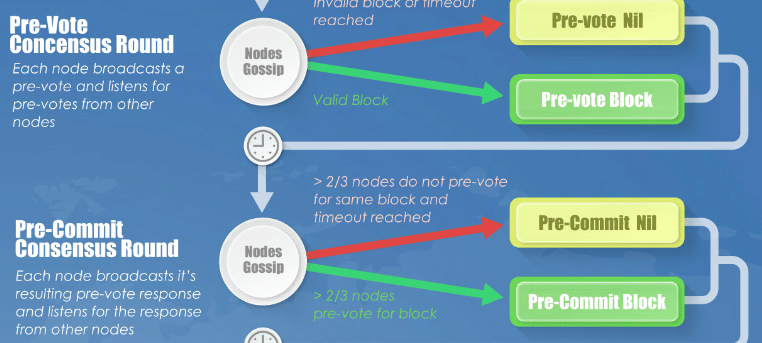
\includegraphics[scale=.43,clip=false]{pictures/tendermint-precommit.png}
  \end{center}

\end{frame}

\begin{frame}\frametitle{Commit}

  \begin{center}
    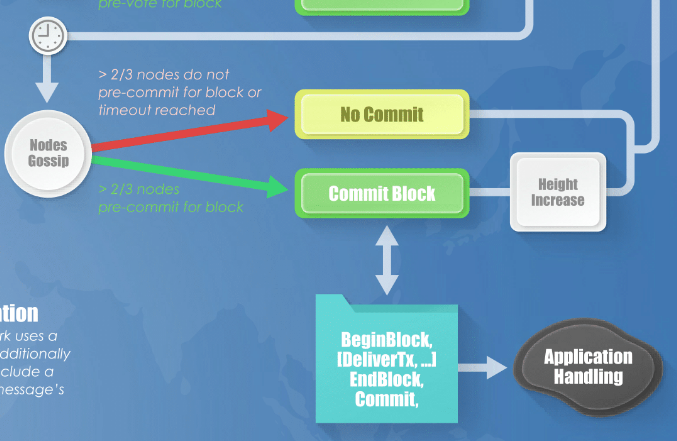
\includegraphics[scale=.38,clip=false]{pictures/tendermint-commit.png}
  \end{center}

  \begin{center}
    \<deliverTx(tx)> executes the transaction \<tx>, hence modifies the state
  \end{center}

\end{frame}

\begin{frame}\frametitle{Next round, or next height}

  \begin{center}
    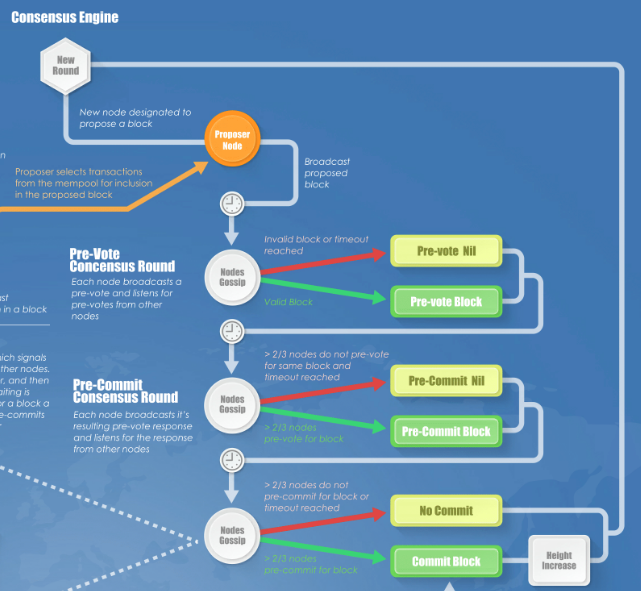
\includegraphics[scale=.36,clip=false]{pictures/tendermint-consensus.png}
  \end{center}

\end{frame}

\begin{frame}\frametitle{Inside a Tendermint block}

  \begin{center}
    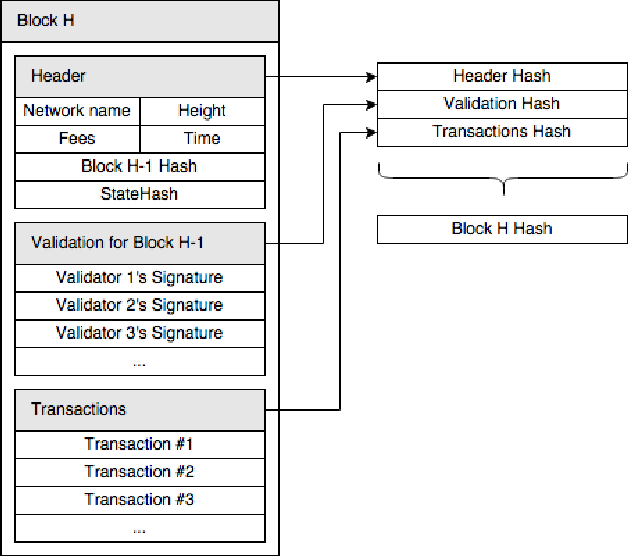
\includegraphics[scale=.38,clip=false]{pictures/tendermint-block.png}
  \end{center}

\end{frame}

\end{document}
